\documentclass[utf8]{beamer}

\usepackage[T1]{fontenc}
\usepackage[brazil]{babel}
\usepackage{sourcecodepro}
\usepackage{minted}
\usepackage[absolute, overlay]{textpos}
\usepackage{changepage} % adjustwidth environment
\usepackage{qrcode}
\usepackage{enumitem}
\usepackage{tikz}


\definecolor{codebgcolor}{HTML}{FFFFFF}
\definecolor{coderulecolor}{HTML}{5F7FFF}
\definecolor{outerbgcolor}{HTML}{FFFFEE}

\setminted{python3, autogobble,
           breaklines, breakanywhere,
           breaksymbolindentleft=0pt, breaksymbolindentright=0pt,
           breaksymbolsepleft=3pt, breaksymbolsepright=3pt,
           breaksymbolright=...,
           bgcolor=codebgcolor, style=borland,
           fontsize=\fontsize{8pt}{8pt},
           frame=lines, rulecolor=coderulecolor, framerule=.7pt}
\setmintedinline{bgcolor={}}

\mode<presentation>
\usetheme{Warsaw}
\usecolortheme{wolverine}
\setbeamercolor{background canvas}{bg=outerbgcolor}
\setbeamercolor{author in head/foot}{bg=black, fg=lightgray}
\beamertemplatenavigationsymbolsempty

\setbeamertemplate{footline}{\leavevmode\hbox{%
  \begin{beamercolorbox}[wd=.31\paperwidth, ht=2.25ex, dp=1ex, center]
                        {author in head/foot}%
    \usebeamerfont{author in head/foot}%
      Danilo J. S. Bellini\hfill\texttt{@danilobellini}%
  \end{beamercolorbox}%
  \begin{beamercolorbox}[wd=.38\paperwidth, ht=2.25ex, dp=1ex, center]
                        {title in head/foot}%
    \usebeamerfont{title in head/foot}%
      Tutorial sobre \insertshorttitle%
  \end{beamercolorbox}%
  \begin{beamercolorbox}[wd=.24\paperwidth, ht=2.25ex, dp=1ex, center]
                        {author in head/foot}%
    \usebeamerfont{author in head/foot}%
      Python Sudeste\hfill%
      \insertshortdate%
  \end{beamercolorbox}%
  \begin{beamercolorbox}[wd=.07\paperwidth, ht=2.25ex, dp=1ex, center]
                        {title in head/foot}%
    \usebeamerfont{title in head/foot}%
      \insertframenumber\,/\,\inserttotalframenumber%
  \end{beamercolorbox}%
}}

\setbeamertemplate{background}{%
  \tikz[overlay,remember picture]%
    \node[opacity=0.05] at (current page.center){%
      \includesvg{.8\paperwidth}{duckdb_logo}%
    };%
}

\title{DuckDB}
\subtitle{Uma revolução pra quem trabalha com dados}
\author{Danilo J. S. Bellini \\ \texttt{@danilobellini}}
\date{2024-07-06}

\setlength{\TPHorizModule}{\paperwidth}
\setlength{\TPVertModule}{\paperheight}

\setitemize{label=\usebeamerfont*{itemize item}%
  \usebeamercolor[fg]{itemize item}%
  \usebeamertemplate{itemize item}%
}

\newcommand{\includesvg}[2]{%
  \ifnum\pdfstrcmp{\pdffilemoddate{#2.svg}}%
                  {\pdffilemoddate{#2.pdf}}>0%
    {\immediate\write18%
     {inkscape -z -D --file=#2.svg --export-pdf=#2.pdf --export-latex}%
    }%
  \fi%
  \centering%
  \resizebox{#1}{!}{%
    \input{#2.pdf_tex}%
  }%
}

\newcommand{\repo}[0]{https://github.com/danilobellini/slides-latex}


\begin{document}


\begin{frame}
  \titlepage
  \center
  {\huge Python Sudeste 2024 @ UFSCar/SP}

  \begin{textblock}{0}(.12, .55)%
    \includesvg{.25\paperwidth}{DuckDB_Logo-horizontal}%
  \end{textblock}
  \begin{textblock}{0}(.67, .5)%
    \colorbox{black}{
      \includesvg{.18\paperwidth}{duckdb_logo}
    }%
  \end{textblock}
\end{frame}


\begin{frame}{RDBMS? OLAP vs OLTP... ACID?}
  \hspace{5ex} O que é o DuckDB?
  \vspace{.5em}
  \begin{itemize}[leftmargin=0mm]
    \item \textbf{Banco de dados} relacional (RDBMS)
    \item OLAP (\emph{OnLine \textbf{Analytical} Processing})
    \begin{itemize}
      \item Otimizado para análise de grandes volumes de dados
      \item Organização interna por ``colunas''
    \end{itemize}
    \item Pode processar carga maior que a memória
    \item Suporta transações ACID
          (Atômicas, Consistentes, Isoladas e Duráveis),
          embora não seja otimizado para OLTP
    \item Muitas possibilidades de integração
          (tipos de arquivos, locais de origem, outros bancos de dados)
    \item Suporta \textbf{SQL} (e um SQL amigável próprio)
    \item \emph{\textbf{In-process}} (roda no processo \emph{host})
    \item Portável (Linux, Windows, macOS, WASM)
    \item Software livre/aberto (licença MIT)
  \end{itemize}
  \tikz[overlay,remember picture]%
    \node[draw, fill=white, rounded corners, inner sep=1pt,
          above=.9em, left=2ex, above left]
      at (current page.south east){%
      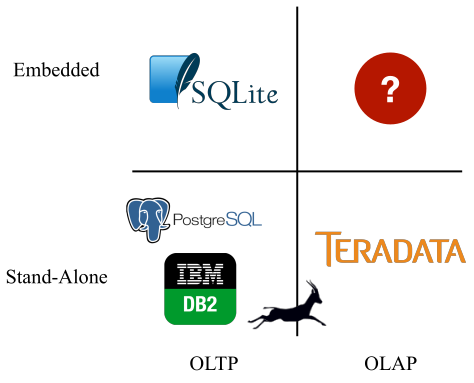
\includegraphics[width=.32\paperwidth]
        {sigmod2019-demo-duckdb-fig1.png}%
    };%
  \tikz[overlay,remember picture]%
    \node[draw, fill=white, rounded corners, inner sep=1pt,
          below=5pt, left=3pt, below left]
      at (current page.north east){%
      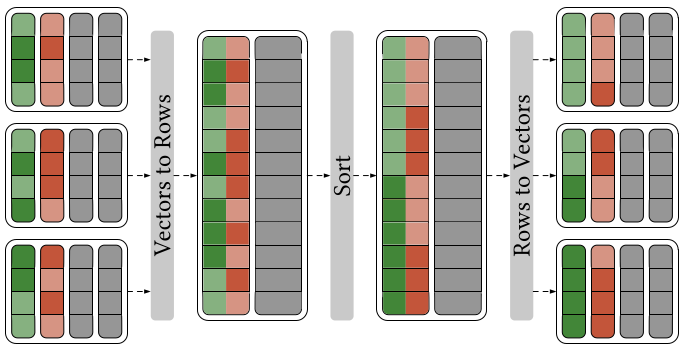
\includegraphics[width=.38\paperwidth]
        {icde2023-kuiper-muehleisen-sorting-fig1.png}%
    };%
\end{frame}


\begin{frame}{Sobre os ombros de gigantes!}
  Inspirado em muitas pesquisas acadêmicas,
  surgiu como parte de pesquisas realizadas na Holanda.
  O ``\emph{may not be obvious at first unless you're Dutch}''
  do PEP-20 (Zen do Python) se encaixa aqui?
  \vfill
  Elementos do \textbf{SQLite} (RDBMS mais usado no mundo)
  que foram trazidos para o DuckDB:
  \begin{itemize}
    \item Não possuir dependências externas (exceto p/ extensões)
    \item Rodar no mesmo processo \emph{host}
    \item Shell/REPL (linha de comando) e testes de lógica SQL
    \item Habilidade em salvar arquivos com extensão ``\texttt{.db}''
          ou manter em memória com o nome ``\texttt{:memory:}''
  \end{itemize}
  \vfill
  O parser SQL é um fork do parser do \textbf{PostgreSQL},
  e diversos elementos de sintaxe são os mesmos,
  como ``\mintinline{sql}{::TIPO}'' para conversões de tipos,
  ``\mintinline{bash}{~}'' e ``\mintinline{bash}{!~}''
  para expressões regulares (POSIX),
  sintaxe para uso de colunas JSON e até mesmo funções.
\end{frame}


\begin{frame}{DuckDB v1.0.0 ``Snow Duck'' (Anas Nivis)}
  \begin{itemize}
    \item Primeira versão estável, lançada em 2024-06-03!
    \item Quase 6 anos de DuckDB (primeiro commit em 2018-07-13)
    \item Licença MIT desde 2018-12-04
    \item Escrito em C++, disponível no PyPI
          (também possui integrações com outras ferramentas/linguagens,
           como o \texttt{dplyr} do R, mas Python possui mais recursos)
  \end{itemize}
  \vfill
  \includesvg{.6\paperwidth}{paddling-of-ducks}
\end{frame}


\begin{frame}[fragile]{Cadê o SQL? \emph{Show me the code}!}
  ``Olá mundo!'' no Shell local ou \url{https://shell.duckdb.org}:%
  \inputminted[lastline=1]{sql}{01_intro.sql}

  Outros exemplos introdutórios:%
  \inputminted[firstline=4, lastline=20]{sql}{01_intro.sql}
\end{frame}


\begin{frame}[fragile]{Tabelas/views em memória; Janela; Arquivos CSV}
  \vspace{-.8em}%
  \inputminted[firstline=23, lastline=50]{sql}{01_intro.sql}
\end{frame}


\begin{frame}[fragile]{E no Python? HTTP?}
  \vspace{-.8em}%
  \inputminted{python}{02_intro.py}
\end{frame}


\begin{frame}[fragile]{Instalação e configuração do ambiente;
                       Exercício!}
  \vspace{-.8em}%
  \inputminted{bash}{03_install.sh}
  \vspace{-2.8em}%
  \inputminted{python}{04_jupysql.py}
  Opcional (DuckDB Shell local): instalar o ``\emph{Command line}'' do
  \url{https://duckdb.org/docs/installation} \qquad ou
  \url{https://repology.org/project/duckdb/versions}
\end{frame}


\begin{frame}[fragile]{Integrações com o Python}
  \inputminted{python}{05_integrations.py}
\end{frame}


\begin{frame}[fragile]{Conectando ao PostgreSQL}
  \vspace{-.8em}%
  \inputminted{python}{06_database.sh}
  \vspace{-2.8em}%
  \inputminted{python}{07_postgres.py}
\end{frame}


\begin{frame}
  \begin{columns}[c]
    \column{.5\textwidth}
    \begin{center}
      {\fontsize{5cm}{2.5cm}\selectfont FIM!}
      \vfill
      \vspace{1em}
      \url{\repo}
      \vfill
      \vspace{1em}
      Para rodar os testes dos slides:
      \mintinline{shell}{python3.8 -m doctest slides.tex}
      \vfill
      \vspace{1em}
    \end{center}
    \vspace{-1em}
    Referências:
    \column{.5\textwidth}
    \begin{center}
      \qrcode[height=5cm]{\repo}
    \end{center}
  \end{columns}
  \vfill
  \fontsize{8pt}{7pt}\selectfont
  \begin{itemize}[label=--, leftmargin=0mm]
    \item \url{https://duckdb.org/docs/}
    \item \url{https://duckdb.org/2024/06/03/announcing-duckdb-100.html}
    \item \url{https://duckdb.org/why_duckdb}
  \end{itemize}
\end{frame}


\end{document}
